\begin{figure}[htbp]
\centering
% Set the overall layout of the tree
\tikzstyle{level 1}=[level distance=4cm, sibling distance=3.5cm]
\tikzstyle{level 2}=[level distance=4cm, sibling distance=2cm]

% Define styles for bags and leafs
\tikzstyle{bag} = [text width=4em, text centered]
\tikzstyle{end} = [circle, minimum width=3pt,fill, inner sep=0pt]
\tikzstyle{fork} = [circle, minimum width=3pt,fill, inner sep=0pt]
% The sloped option gives rotated edge labels. Personally
% I find sloped labels a bit difficult to read. Remove the sloped options
% to get horizontal labels. 
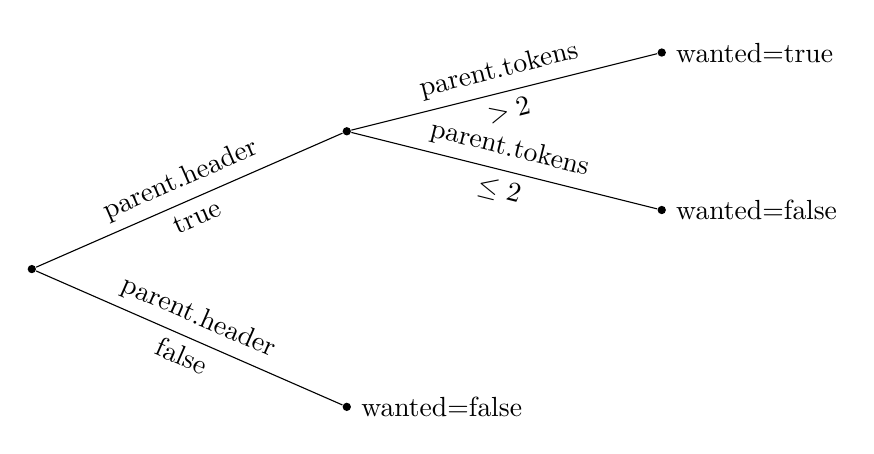
\begin{tikzpicture}[grow=right, sloped]
\node[fork] {}
    child {
        node[end, label=right:
                    {\url{wanted=false}}]{}      
	edge from parent 
            node[above] {\url{parent.header}}
            node[below]  {\url{false}}
    }
    child {
        node[fork]{}   
        child {
                node[end, label=right:
                    {\url{wanted=false}}] {}
                edge from parent
                node[above] {\url{parent.tokens}}
                node[below]  {$\leq 2$}
            }
            child {
                node[end, label=right:
                    {\url{wanted=true}}] {}
                edge from parent
                node[above] {\url{parent.tokens}}
                node[below]  {$>2$}
            }
        edge from parent         
            node[above] {\url{parent.header}}
            node[below]  {\url{true}}
    };
\end{tikzpicture}
\caption{Decision tree generated when search entries on Google are selected.}
\label{fig:decisiontree}
\end{figure}